% !TEX output_directory=output
\documentclass{beamer}

\usepackage[beamer]{kaufman}

\bibliography{../refs.bib}
\graphicspath{{../graphics/}}

\title{Hamiltonian Engineering via Reinforcement Learning}
\author{Will Kaufman}
\institute{Ramanathan Group \\ Dartmouth College}

\titlegraphic{\includegraphics[height=.1\textheight]{LonePine.pdf}}

\begin{document}

\frame{\titlepage}

\begin{frame}
\frametitle{Table of Contents}
\tableofcontents
\end{frame}

\section{Hamiltonian engineering}

\begin{frame}
\frametitle{Hamiltonian engineering}

Hamiltonian engineering seeks to control the system's evolution so that it appears to evolve under a target ``effective'' Hamiltonian.

\begin{equation}
    H(t) = H_\text{system} + H_\text{control}(t)
\end{equation}

\begin{equation}\label{eq:strob_measure}
    \rho(Nt_c) = U_\text{target}(Nt_c) \rho(0) U_\text{target}^\dagger(Nt_c)
\end{equation}

\pause

In NMR \cite{1976ii}\dots

\begin{align}\label{eq:ham_spin}
    H_\text{system} &= \sum_i \delta_i I_z^i + \sum_{i,j} d_{ij} \left( 3I_z^iI_z^j - \mathbf{I^i} \cdot \mathbf{I^j} \right)
    = H_\text{CS} + H_\text{D} \\
    H_\text{control}(t) &= -B_1(t) \sum_i \gamma_n^i I_x^i
\end{align}

\end{frame}

\section{Previous approaches}

\begin{frame}
\frametitle{Average Hamiltonian theory}

Average Hamiltonian theory is one approach to solving the Hamiltonian engineering problem
\cite{PhysRev.175.453}.
If a pulse sequence with cycle time is both cyclic and periodic
\cite{gerstein-dybowski}
\begin{align}\label{eq:AHT_conditions}
    U_\text{rf}(t_c) &= T\exp \left(
        -i \int_0^{t_c} H_\text{rf}(t) dt \right) = \pm \identity
        & \text{(cyclic)} \\
    H_\text{rf}(t) &= H_\text{rf}(t + Nt_c) & \text{(periodic)}
\end{align}
then, using the Magnus Expansion, the propagator can be given by
\begin{align}\label{eq:AHT_average}
    U(t_c) &= \exp\left( -i t_c (\overline{H}^{(0)} +
        \overline{H}^{(1)} + \dots) \right) \\
    \overline{H}^{(0)} &= 1/t_c \int_0^{t_c}
        U_\text{rf}(t) H_\text{int} U_\text{rf}^\dagger(t) dt
\end{align}

\end{frame}

\begin{frame}
\frametitle{Average Hamiltonian theory: examples}

To engineer a target Hamiltonian $H_t$, the pulse sequence is chosen so that $\overline{H}^{(0)} = H_t$. Higher-order terms $\overline{H}^{(1)}, \overline{H}^{(2)}, \dots$ can also be considered (e.g. symmetrization).

~

\begin{tabularx}{\linewidth}{c c c}
    Name & Pulse sequence (left to right) & $\overline{H}^{(0)}$ \\
    \hline
    WHH-4 \cite{PhysRevLett.20.180} &
        $\tau, P_{-x}, \tau, P_y, \tau, \tau, P_{-y}, \tau, P_x, \tau$ &
        $\frac{1}{3} \sum_i \delta_i \left( I_x^i + I_y^i + I_z^i \right)$ \\
    MREV-8 \cite{mansfield1971symmetrized} &
        $\tau, P_{-x}, \tau, P_y, \tau, \tau, P_{-y}, \tau, P_x, \tau$,
        $\tau, P_{x}, \tau, P_y, \tau, \tau, P_{-y}, \tau, P_{-x}, \tau$ &
        $\frac{1}{3} \sum_i \delta_i \left( I_x^i + I_z^i \right)$ \\
    HoRD-qubit-5 \cite{O_Keeffe_2019} &
        $\tau, P_y, \tau, P_x^2, \tau, P_x P_y P_{-x}^2$,
        $\tau, P_{-x} P_y P_{-x}, \tau, P_y P_x, \tau$ &
        $1/3 \sum_i I_z^i$ \\
    \hline
\end{tabularx}

Pulse sequences for dipolar decoupling of spin-1 systems exist \cite{PhysRevLett.119.183603, O_Keeffe_2019}.

\end{frame}

\begin{frame}
\frametitle{Average Hamiltonian theory: benefits and limitations}

\begin{itemize}
    \item Analytically tractable
    \item Account for finite-width pulses
    \item Can characterize terms in average Hamiltonian
    \pause
    \item Only tractable for lowest-order terms
    \item Enforced structure on pulse sequences
\end{itemize}

\end{frame}

\begin{frame}
\frametitle{GRAPE}

% TODO include GRAPE here

\end{frame}

% TODO add benefits/limitations of GRAPE?

\section{Reinforcement learning as alternative approach}

\begin{frame}
\frametitle{Reinforcement learning paradigm}

% TODO intro section to RL, relate to MDP?

\begin{figure}
    \centering
    \scalebox{.5}{
    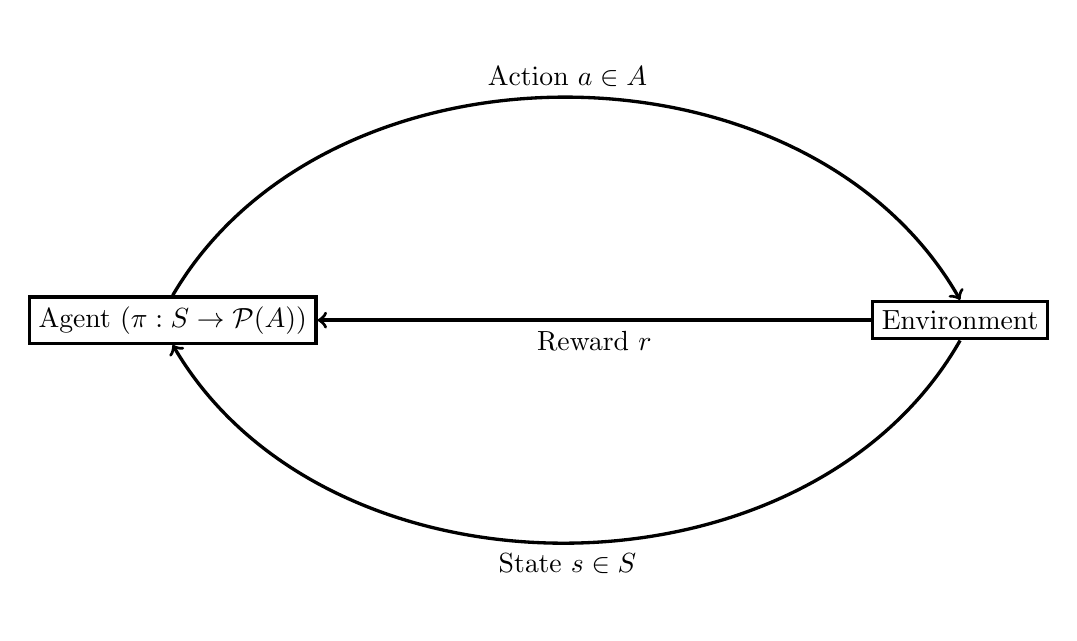
\begin{tikzpicture}[->, very thick]
         %nodes
         \node[draw] at (-5,0) (agent) {Agent ($\pi: S \to \mathcal{P}(A)$)};
         \node[draw] at (5,0) (env) {Environment};
         \path
             (agent.north) edge[bend left=60] node[above] {Action $a \in A$} (env.north)
             (env.south) edge[bend left=60] node[below] {State $s \in S$} (agent.south)
             (env.west) edge node[below] {Reward $r$} (agent.east);
    \end{tikzpicture}
    }
    %\caption{The general reinforcement learning paradigm.}
    \label{fig:RL}
\end{figure}

\end{frame}

\begin{frame}
\frametitle{RL Definitions}

\begin{itemize}
    \item State space $S$; all possible states of the environment
    \item Action space $A$: all possible actions that can be performed
    \item Total return $R_t$: sum of all rewards from time $t$ to end of episode (length $T$)
    \begin{equation}\label{eq:return}
        R_t = \sum_{k=t}^T r_k
    \end{equation}
    \pause
    \item Stochastic policy $\pi: S \to \mathcal{P}(A)$:
        maps from states to probability distributions over actions (also written $\pi(a|s)$)
    \item State value $V^\pi:S \to \R$: expected return from state following policy $\pi$
    \item State-action value $Q^\pi: S \times A \to \R$: expected return from state and performing action, then following policy $\pi$
\end{itemize}

\end{frame}

\begin{frame}
\frametitle{Actor-critic methods}

A ``critic'' learns the value function $V^\pi_\phi$, and an ``actor'' learns the policy function $\pi_\theta$ \cite{sutton2018reinforcement}.

\begin{align}\label{eq:loss_fns}
    L(\phi) &= \sum_i (\hat{R}_i - V^\pi_\phi(s_i))^2 \\
    L(\theta) &= -\sum_i (\hat{R}_i - V^\pi_\phi(s_i))
        \ln \pi_\theta(a_i|s_i)
\end{align}

$\hat{R}_i - V^\pi_\phi(s_i)$ is called the \emph{advantage} $A_i$.
% TODO include Bellman equation?

\pause

Gradient-based methods are susceptible to local minima.

\end{frame}

\begin{frame}
\frametitle{Evolutionary reinforcement learning}

% TODO diagram

\end{frame}

\begin{frame}
\frametitle{Applying RL to Hamiltonian engineering}

% TODO make a table?
%How things relate

\end{frame}

\section{Results}

\begin{frame}
\frametitle{Hyperparameter search and algorithm performance}
% TODO
\end{frame}

\begin{frame}
\frametitle{Hyperparameter search and algorithm performance (cont.)}
% TODO
\end{frame}

\begin{frame}
\frametitle{Candidate pulse sequences}

% TODO
% general evaluation strategy (compare to WHH-4, MREV-8)
% compare on similar timeframe
% robustness?
% simulation parameters

\end{frame}

\begin{frame}
\frametitle{Candidate pulse sequences (cont.)}
% TODO
\end{frame}

\section{Next steps}

\begin{frame}
\frametitle{Improvements to RL algorithm}
% TODO
% convergence, speed, robustness, efficiency
% change setup to GRAPE-like tests (likely won't be as effective)
\end{frame}

\begin{frame}
\frametitle{Experimental verification of candidate pulse sequences}
% TODO
\end{frame}

\begin{frame}[allowframebreaks]
\frametitle{Bibliography}

\printbibliography

\end{frame}






\end{document}
